\chapter{Distributed Document Embeddings}
\label{chapter:distembed}
In this chapter we describe the concept of distributed word and document embeddings and why distributed representations of words and documents are better than one-hot or bag-of-words representations as described in \ref{sec:textrepr}. We then give a background on different models that learn distributed representations for words in a fully unsupervised manner and finally describe in detail our proposed model for learning distributed embeddings for documents that can be used for multi-label text classification.

\section{Motivation}
\label{sec:motivation_distributed}
\todo{Get in tune to document representations. Say words and documents suffer in the same manner with one-hot or bow representations. Express problems in docs with changing words. Give example of sentence}

\todo{Can be tackled with distributed repr. Similarity measures as simple as cos-distance can be introduced in documents. Lets model joint distributions of words with continuous distributions. Words have distributed representaions but not docs. }

Words are regarded as atomic symbols in most rule-based and statistical natural language processing(NLP) tasks and hence need the appropriate representation to solve the NLP tasks with greater ease and accuracy. 
Words are traditionally expressed as one-hot vectors, i.e. as vectors of the size of the vocabulary where exactly one element is $1$ and the rest all are zero.
Though these representations have been widely used, one-hot representations have a plethora of drawbacks that pose problems and limit the ability of systems to perform better. 
\begin{enumerate}
\item \textbf{Curse of Dimensionality} : One-hot representations lead word vectors to be the size of the vocabulary which often consists of tens to hundreds of thousands of words. Due to this curse of dimensionality, language modeling becomes almost impossible where the number of parameters would grow exponentially with the size of the vocabulary if the words are represented as one-hot vectors.

\item \textbf{No Word Similarity} : As words are represented by sparse orthogonal vectors, there is no notion of word similarity that can be introduced. In one-hot representation, the word ``symphony'' is equally close to the words ``bark'' and ``guitar''. We would want word representations such that they capture the semantic or topical similarity between words.
\end{enumerate}

Due to the problems discussed above there is a need for more robust, low-dimensional, non-sparse vector representations for words that capture the semantic similarity between them, can be used to model language with continuous distributions and can be used as inputs for various other NLP tasks. 

\section{Background on Word Embeddings}
\label{sec:background_distributed}
Distributed word representations are dense fixed-sized feature vectors learned for words in an unsupervised manner from large text corpus that capture the semantic similarity between words. Each word $w_{i}$ in the corpus is represented by a vector, $v_{w_{i}} \in \mathbb{R}^{m}$, where $m$ usually ranges from $50-300$. These dense representations help deal with sparsity and high-dimensionality issues in one-hot representations and also provide provision for estimating similarities between words; which is as simple as taking the dot-product or calculating the cosine-distance between the vectors. 

All of the word vector learning models make use of neural networks  ( \citep{bengio2003neural}, \citep{mnih2013learning}, \citep{mikolov2013distributed}, \citep{collobert2011natural}, \citep{bottou2014machine}, \citep{turian2010word}, \citep{levy2014dependencybased} ) but differ in their training objectives. 

Below we describe in detail two models to show how models with very different learning objectives and architecture can lead to learning high-quality word vectors.

\subsection{Neural Probabilistic Language Model (NPLM)}
\label{sec:bengio}
Introduced by \cite{bengio2003neural}, their model aims to learn distributed word vectors and a probability function that uses these vectors to learn a statistical model of language. In their model, the probability of a word sequence is expressed as the product of conditional probabilities of the next word given the previous ones. 
\begin{equation}
P(w_{1}^{T}) =  \prod_{t=1}^{T} P(w_{t}| w_{1}^{t-1})
\end{equation}
And making the n-gram assumption, 
\begin{equation}
P(w_{t} | w_{1}^{t-1}) \approx P(w_{t} | w_{t-n+1}^{t-1})
\end{equation}
i.e. the probability of the next word in the sequence is mostly affected by the local context, in this the previous $n$-words and not the whole past sequence.

Their model maps each word to a $m$-dimensional vector in a matrix $C \in \mathbb{R}^{|V|\times m}$ and estimates the probability $P(w_{t} = i|w_{t-n+1}^{t-1})$ i.e. the probability that the $t^{th}$ word in the sequence is $w_{i}$. The neural network that is used to estimate this probability using the word vectors is shown in Figure~\ref{fig:nn:bengio}
\begin{figure}[t!]
    \centering
        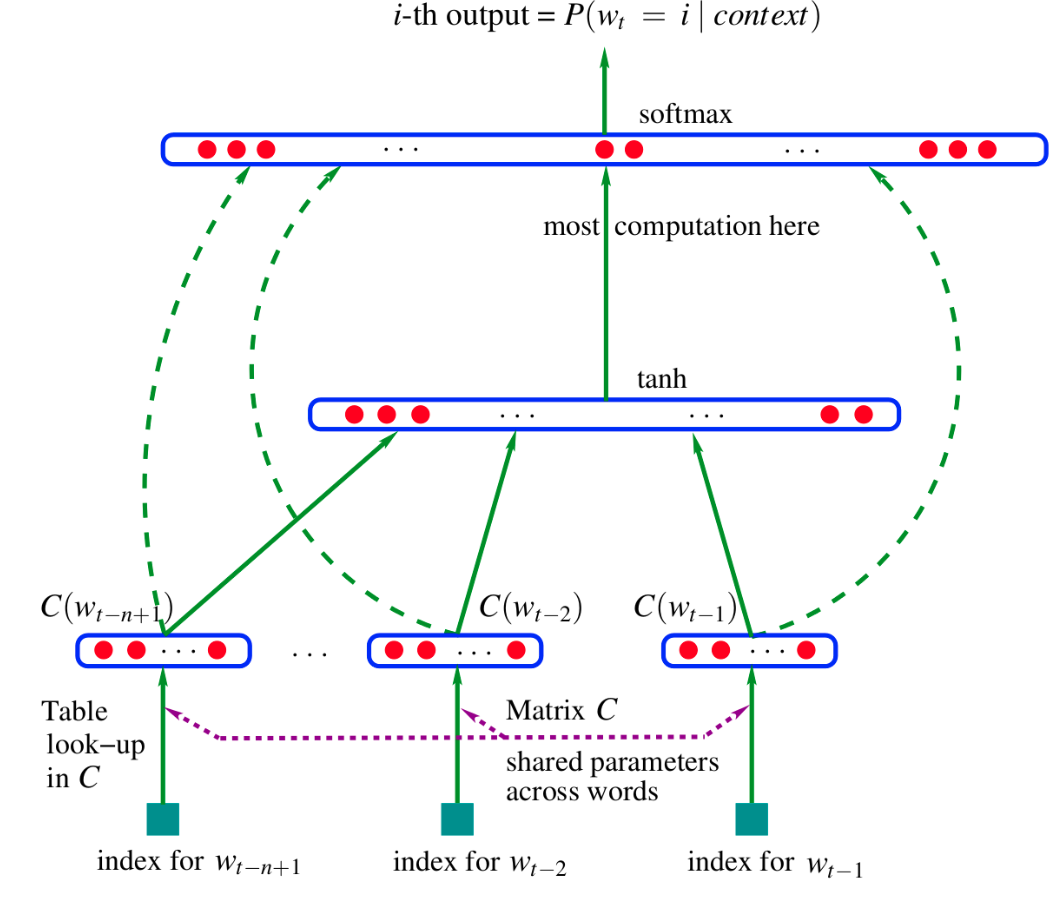
\includegraphics[width=0.8\textwidth]{figs/bengio_nn.png}
    \caption{Bengio's Neural Network Architecture for Neural Probabilistic Language Model}
    \label{fig:nn:bengio}
\end{figure}
For each input sequence, the neural network outputs a vector $y \in \mathbb{R}^{|V|}$, where $y_{i}$ is the unnormalized log-probability that the $t^{th}$ word in the sequence is $w_{i}$.
\begin{equation}
y = b + Wx + Utanh(d + Hx)
\end{equation}
where $tanh$ is the hyperbolic tangent applied to introduce non-linearity and $x$ is the word feature layer activation vector constructed by the concatenation of the context word vectors,
\begin{equation}
x = (C(w_{t-1}), C(w_{t-2}), \ldots, C(w_{t-n+1}))
\end{equation}
The unnormalized log probabilities in $y$ are converted to positive probabilities summing to $1$ by using a \emph{softmax} output layer that computes, 
\begin{equation}
P(w_{t} = i | w_{t-1}, \ldots, w_{t-n+1}) = \frac{e^{y_{w_t}}}{\sum_{i}e^{y_{i}}}
\end{equation}
The parameters of the model $(b, d, W, U, H)$ and the word vectors $C$ are estimated by maximizing the log-likelihood of the training corpus.

\subsection{Log-Linear Models : word2vec}
\label{sec:word2vec}
Simple log-linear models are proposed in \cite{mikolov2013efficient} as opposed to the non-linear NPLM model to bring down the training time complexity without sacrificing with the quality of the word vectors. \todo{Also these models are based on the Distributional Hypothesis} The models bring down the complexity of learning vectors by not having a non-linear layer and matrix weighting of the input vectors that are the costliest operations in NPLM. The two models proposed in \cite{mikolov2013efficient} are Continuous Bag-of-Words and Continuous Skip-Gram model, described below.

\subsubsection{Continuous Bag-of-Words (CBOW)}
\label{sec:cbow}
This model is different from the NPLM in that the projection layer is shared for all words; i.e. all words get projected into the same hidden layer vector (their vectors are averaged). This architecture hence neglects the ordering of the words as opposed to NNLM that uses the concatenation of input vectors for the projection layer. The training criteria in this model is to to classify the current (middle) word given its context. It also uses word sequence from the future to aid this task with the relaxation that the aim is not to learn a language model. The model architecture is given in Figure~\ref{fig:nn:cbow}.
\begin{figure}[h!]
    \centering
        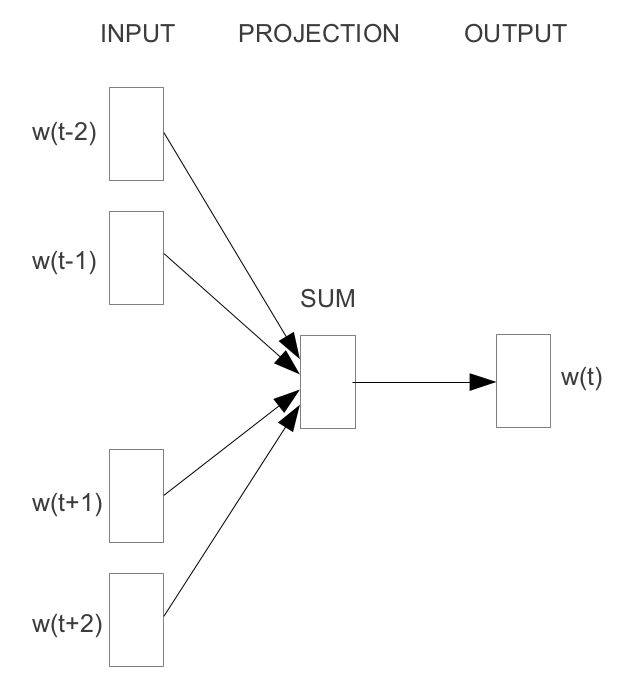
\includegraphics[width=0.5\textwidth]{figs/mikolov_cbow.png}
    \caption{Continuous Bag-of-Words Model (CBOW) \todo{Add ref?}}
    \label{fig:nn:cbow}
\end{figure}
The model first computes the hidden layer vector $h$, 
\begin{equation}
h(w_{t-k}, \ldots, w_{t+k}) = \frac{w_{t-k} + \ldots + w_{t-1} + w_{t+1} + \dots + w_{t+k}}{2k}
\end{equation}
where, $w_{t-i}$ is the $i$-th previous word in the context of the middle word $w_{t}$ and $k$ is the window length.
The neural network then computes a unnormalized log-probability vector $y$ similar to Sec.\ref{sec:bengio}, and uses the \emph{softmax}-classifier to estimate $P(w_{t}|w_{t-k}, \ldots, w_{t+k})$,
\begin{equation}
y = b + Uh(w_{t-k}, \ldots, w_{t+k})\\
\end{equation}
\begin{equation}
\label{eq:cbow:prob}
P(w_{t}|w_{t-k}, \ldots, w_{t+k}) = \frac{e^{y_{w_t}}}{\sum_{i} e^{y_{i}}}
\end{equation}
The parameters of the CBOW model, $(b, U)$ and the word vectors ($w_{i}$) are learned by maximizing the average log probability (Eq.~\ref{eq:cbow:prob}) of the training corpus.

\subsubsection{Continuous Skip-gram}
This model is similar to the CBOW model, but instead of predicting the middle word based on the context, it tries to maximize the classification of a word based on another word in the context. More precisely, given each word, the skip-gram model tries to predict words within a certain range before and after the current word. The model architecture is given in Figure~\ref{fig:nn:skip}
\begin{figure}[h!]
    \centering
        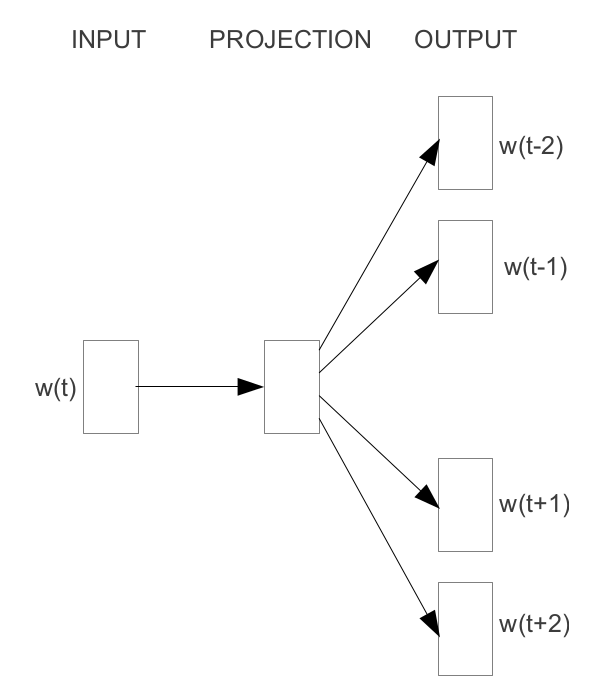
\includegraphics[width=0.4\textwidth]{figs/mikolov_skip.png}
    \caption{Continuous Skip-gram Model \todo{Add ref?}}
    \label{fig:nn:skip}
\end{figure}
Formally, given a sequence of words in a context $w_{t-k}, \ldots, w_{t+k}$, the skip-gram model defines $P(w_{t+j}|w_{t})$ using the \emph{softmax}-classifier in the following manner,
\begin{equation}
\label{eq:skip:prob}
P(w_{t+j}|w_{t}) = \frac{e^{(v_{w_{t}} \cdot v_{w_{t+j}} )} }{\sum_{i} e^{(v_{w_{t}} \cdot v_{w_{i}})} }
\end{equation}
The only parameters of the Skip-gram model are the word vectors ($v_{w_{i}}$) that are learned by maximizing the average log probability (Eq.~\ref{eq:skip:prob}) of predicting all the context words for all the words in the training corpus.

The CBOW and the Skip-gram models use the \emph{hierarchical softmax} \citep{morin2005hierarchical} instead of the full softmax to speed-up the learning process.

The quality of the word vectors is tested using the \emph{Semantic-Syntactic Word Relationship test} that evaluates the model performance on retrieving semantically and syntactically similar words to the given test words. The word vectors learned using the skip-gram model are also shown to encode many linguistic regularities and pattern \citep{mikolov2013linguistic} and show additive compositionality using simple vector arithmetics. For example, the result of the vector calculation $vec(Madrid) - vec(Spain) + vec(France)$ is closest to $vec(Paris)$ than any other word vectors.

\subsubsection{Dependency-based Word Embeddings}
Instead of using bag-of-words based context as used in \emph{NPLM} and \emph{word2vec}, \cite{levy2014dependencybased} use arbitrary contexts to investigate its effects on the word vectors and the properties they encode. The most important of their techniques is to derive the contexts based on the syntactic relations that the word participates is. For each word $w$ and its modifiers $m_1, \ldots, m_k$ found using the parse tree of the sentence, contexts $(m_{1}, lbl_{1}, \ldots, m_{k}, lbl_{k})$ are extracted, where $lbl$ is the type of the dependency relation between word and the modifier and $lbl^{-1}$ is used to mark the inverse-relation. An example of the contexts extracted for a sentence is given in Figure~\ref{fig:dep:context}.
\begin{figure}[h!]
    \centering
        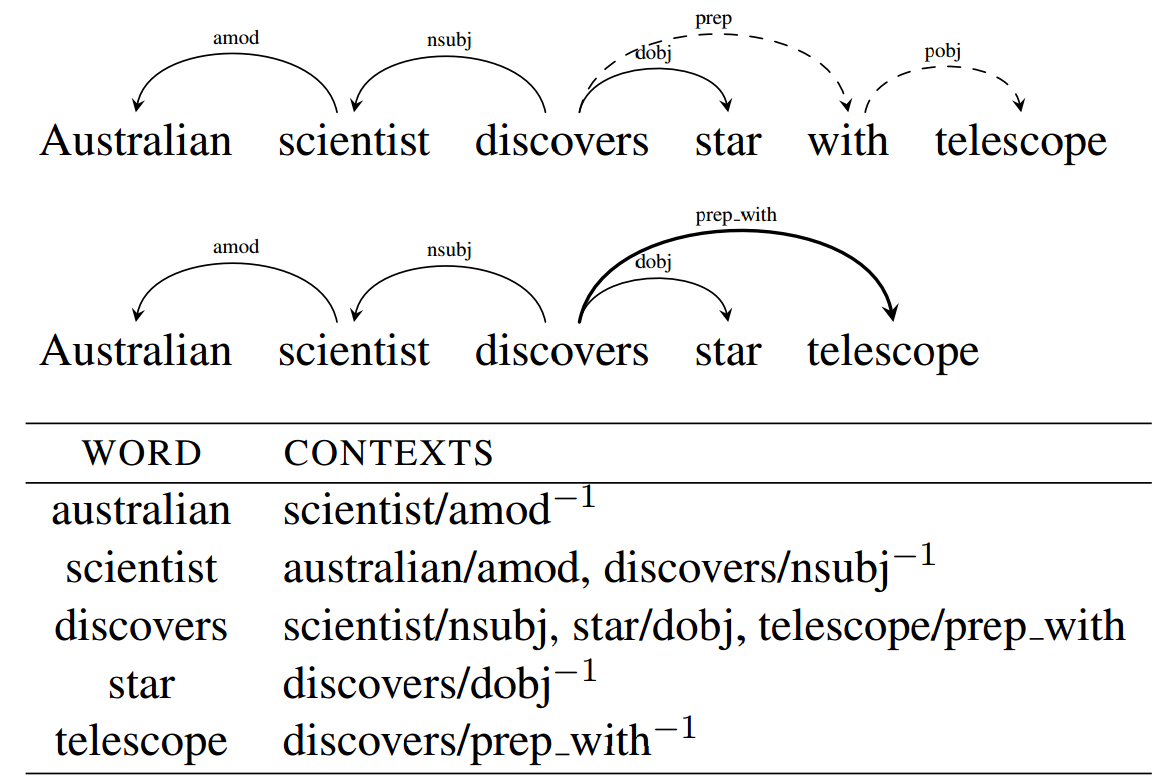
\includegraphics[width=0.7\textwidth]{figs/dependency_context.png}
    \caption{Dependency-based context extraction example \todo{Add ref?}}
    \label{fig:dep:context}
\end{figure}
After extracting the contexts, their model uses the neural network architecture and the training objective of the skip-gram model to learn word vectors. On comparison to the vectors learned from the skip-gram model on the tasks of \emph{topical similarity} and \emph{functional similarity} estimation, it is found that the vectors learned from this model perform better on the \emph{functional similarity} task that expects word vectors to encode syntactic relationships better. In the task of \emph{topical similarity} estimation, the vectors from the skip-gram model performed better as they encode semantic similarity between words because of the bag-of-words context used during training.

\section{Document Embeddings}
\label{sec:document_embeddings}
In the previous section we saw how distributed word embeddings that encode semantic similarity can be learned from text. 
Though these semantic word spaces are very useful for a lot of tasks, their ability to capture the complexity and compositionality of human language is limited. 
Word embeddings cannot be directly used to represent longer phrases, sentences and documents to express their meaning. 
Tasks such as word sense disambiguation, sentiment analysis, text categorization etc. all require the text representation to capture the semantic content of the text for better inputs to learning algorithms as compared to a simple bag-of-words model. 

Progress towards learning distributed representations for longer pieces of text, such as phrase-level or sentence-level representations [\cite{mitchell2010composition}, \cite{zanzotto2010estimating}, \cite{yessenalina2011compositional}, \cite{grefenstette2013multi}, \cite{mikolov2013distributed}] that capture semantic compositionality has been promising, but most models do not go beyond simple weighted average of word vectors to represent longer texts. 
\cite{socher2013recursive} proposes a more sophisticated approach using recursive tensor neural network where the dependency parse-tree of the sentence is used to compose word vectors in a bottom-up approach to represent sentences for sentiment classification of phrases and sentences. 
Both the techniques have weaknesses for learning document representations. The first approach is analogous to a bag-of-words approach and neglects word order while representing documents whereas the second approach considers syntactic dependencies but cannot go beyond sentences as it relies on parsing.

%\subsection{Learning Document Embeddings : Our Approach}
Below we present our model on learning universal distributed vector representations for documents and words in the corpus such that,
\begin{enumerate}
\item The learned vectors encode semantic and topical content of the documents and words.
\item Semantically similar documents/words have similar vector representations.
\end{enumerate}
%Our model is inspired by the work on continuous bag-of-words model \citep{mikolov2013efficient} and \citep{le2014distributed} model of learning representations for sentences and paragraphs. 
To learn vectors that satisfy $1.$ and $2.$ above, we hypothesize that document representations should be learned such that they can aid in the prediction of words in a given word sequence from the document. In the sections below we formally introduce the problem and present our model to learn document and word vector representations.

\subsection{Problem Setup}
Given a set of documents, $\setD=\{d_{1}, \ldots, d_{|\setD|}\}$ and a vocabulary of words, $\setW$ constructed using the set of documents, we wish to embed each document $d_{i} \in$ \setD and each word in the vocabulary onto the same $k$-dimensional space such that the learned vectors encode semantic content of the entities. 

For every sequence of words $w_{t-c}, \ldots, w_{t+c}$ in, say document $d_{i}$, we wish to estimate the probability $p(w_{t}|d_{i}, w_{t-c}, \ldots, w_{t-1}, w_{t+1}, \ldots, w_{t+c})$ of predicting the middle word in the sequence using the information about the document and the words in the context. 
We will estimate this probability using the vector representations for documents and words and learn vectors such that the probability of predicting the middle word in the context correctly is maximized.

\subsection{Our Model}
\label{sec:docem_ourmodel}
A document $d_{i} \in \setD$, indexed by `$i$', in our model is represented by a vector $\vecdi{i} \in \mathbb{R}^{k}$, which is also the $i$-th column of the matrix $\matD = \left[\vecdi{1}, \ldots, \vecdi{|\setD|}\right] \in \mathbb{R}^{k \times |\setD|}$. 
Similarly, a word indexed by `$i$' in the vocabulary $\setW$ is represented by vector $\vecwi{i} \in \mathbb{R}^{k}$, which is also the $i$-th column of the matrix $\matW = \left[\vecwi{1}, \ldots, \vecwi{|\setW|}\right] \in \mathbb{R}^{k \times |\setW|}$.

Given a sequence $(w_{t-c}, \ldots, w_{t+c})$ of $2c+1$ words and the document it occurs in, our training objective is to maximize the probability of correctly predicting the middle word $w_{t}$ using the surrounding context words $(w_{t-c}, \ldots, w_{t-1}, w_{t+1}, \ldots, w_{t+c})$, which we now denote as $context$ as a shorthand, and the information about the document in terms of their distributed vector representations. 
Therefore, our training objective is to maximize the probability $p(w_{t} | d_{i}, context)$ of correctly predicting the middle word using the information about the surrounding words and the document the sequence occurs in. 

To learn distributed word and document representations, we present a neural network model using which we,
\begin{enumerate}
\item Represent each word and document in the corpus by a $k$-dimensional distributed representation stored as vectors in the matrices $\matW$ and $\matD$, respectively.
\item Estimate the probability of predicting the middle word in a sequence, given the document it occurs in, using the vector representation of the document and the words in the context.
\item Learn the word and document vectors simultaneously with the parameters of the function to estimate the probability.
\end{enumerate}
The architecture for the proposed neural network is given in Fig.~\ref{fig:nn:archi}.
Also note that the word vector representations learned and stored in the matrix $\matW$ are universal representations and shared across all documents and contexts.
\begin{figure}[h!]
    \centering
        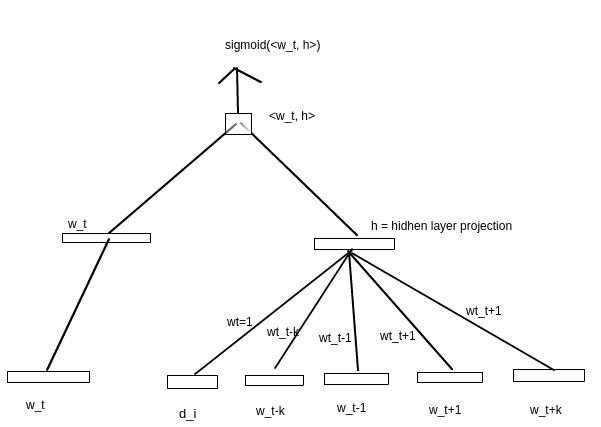
\includegraphics[width=0.9\textwidth]{figs/nn_arch.png}
    \caption{GloDETC : Neural Network Architecture \todo{Change figure}}
    \label{fig:nn:archi}
\end{figure}

%\para{Projection Layer (Context Representation)} : 
\subsubsection{Projection Layer (Context Representation)}
We represent the context(words surrounding the middle word to be predicted) and the document together in the same projection layer, denoted by $h_{c} \in \mathbb{R}^{k}$, by taking a weighted sum of the corresponding vector representations. 
The weights for the context words $\Lambda = \{\wgt{i} | i=\{t-c, \ldots, t-1, t+1, \ldots, t+c\}\}$ are kept universal for different sequences across the corpus as we expect the weights to learn some kind of syntactic quality of the language to better represent the context. Also the weight corresponding to the document vector is kept constant at $1$ as we expected the document to have equal contribution to all sequences. This also gave the best results.
We also (unsuccessfully) experimented by taking matrix weights instead of scalar weights($\wgt{i}$) to learn better syntactic qualities of the language. 

\begin{equation}
\label{eq:hidden_vec}
h_{c} = \vecdi{i} + \wgt{t-c}\vecwi{t-c} + \ldots + \wgt{t-1}\vecwi{t-1} + \wgt{t+1}\vecwi{t+1} + \wgt{t+c}\vecwi{t+c}
\end{equation}

%\textbf{Probability Prediction} : 
\subsubsection{Estimating Prediction Probability}
We expect in absence of any non-linearity that the projection layer vector should be aligned to the correct middle word of the sequence. Hence we estimate the probability of predicting the word $w_{t}$ as the middle word in the following manner. 
\begin{enumerate}
\item An output score $s_{w_{i}} \in \mathbb{R}$ for every $w_{i}$ in the vocabulary is estimated by,
\begin{equation}
\label{eq:nn_score}
s_{w_{i}} = \sigma(\vecwi{w_{i}}\cdot h_{c})
\end{equation}
where $\sigma(z) = \frac{1}{1+e^{-z}}$ is the standard sigmoid function. 
\item After calculating the score for each of the word in the vocabulary, we use the \emph{softmax} classifier to estimate the probability of predicting the actual correct word $w_{t}$ as the middle word in the sequence,
\begin{equation}
\label{eq:soft_prob}
p(w_{t} | d_{i}, w_{t-c}, \ldots, w_{t-1}, w_{t+1}, \ldots, w_{t+c}) = \frac{e^{s_{w_{t}}}}{\sum_{i \in \setW} e^{s_{i}}}
\end{equation}
\end{enumerate}

%\textbf{Training Objective} : 
\subsubsection{Training Objective}
The training data $\traindata$, is composed of $M$ training sequences each of which consists a $2c+1$ length sequence of words and the document index it belongs to. For example, $t = \{d^{(m)}_{i}, w^{(m)}_{t-c}, \ldots, w^{(m)}_{t+c}\}$ represents the $m^{th}$ training sequence in $\traindata$.  

Given the training data $\traindata$, our objective is to learn an optimum parameter set $\Theta = (\matD, \matW, \Lambda)$ consisting of the document and word vector matrices and the projection layer weights for the context words, by maximizing the average log probability of estimating the middle word correctly in all the training word sequences where the probability of estimating the middle word as $w_{i}$ is given by Eq.~\ref{eq:soft_prob}. Therefore, 
\begin{equation}
\label{eq:paramter_argmax}
\hat{\Theta} =  \argmax_{\Theta}~l(\traindata, \Theta)
\end{equation}
\begin{equation}
\label{eq:training_objective}
l(\traindata, \Theta) = \frac{1}{M}\sum_{m=1}^{M} \log \left[p(w^{(m)}_{t} | d^{(m)}_{i}, w^{(m)}_{t-c}, \ldots, w^{(m)}_{t-1}, w^{(m)}_{t+1}, \ldots, w^{(m)}_{t+c})\right]
\end{equation}
To learn the optimize the above training objective, we can use the Stochastic Gradient Descent(SGD) algorithm to find gradient of the objective function (Eq.~\ref{eq:training_objective}) w.r.t. to the individual parameters $\theta_{i}$ and apply the update rule as follows,
\begin{equation}
\label{eq:update_theta}
\theta^{(x)}_{i} = \theta^{(x-1)}_{i} + \gamma\frac{\partial l(\traindata, \Theta)}{\partial \theta_{i}}
\end{equation}
where $x$ is the current iteration number and $\gamma$ is the learning rate. Also note that we add the gradient to $\theta^{(x)}_{i}$ because we wish to maximize the training objective.
Updating the parameters for sufficient number of iterations should yield the optimum document and word vectors along with the weights for the neural network.

\subsubsection{Noise Contrastive Estimation (NCE)}
As we see in Eq~\ref{eq:soft_prob}, estimating the probability for each training word sequence requires a sweep through the whole vocabulary of size $|\setW|$ which can be a very expensive computation given that typical vocabulary sizes range from a few tens to a few hundreds of thousand words for large datasets. Approaches to reduce this training time, such as, use of hierarchical soft-max \citep{morin2005hierarchical} and use of importance sampling to approximate the likelihood gradient \citep{bengio2003quick}, \citep{bengio2008adaptive} have been proposed. Using hierarchical softmax reduces the training time from linear to logarithmic in vocabulary size but is considerable more involved and finding well-performing trees is not trivial. Also, though importance sampling provides substantial speedups, it suffers from stability problems.

\textbf{Noise Contrastive Estimation (NCE)} \citep{gutmann2012noise} is method for fitting unnormalized probabilities by reducing the problem of \emph{density estimation} to \emph{probabilistic binary classification}. It has also been adapted to NPLM (Sec.~\ref{sec:bengio}) \citep{mnih2012fast} and learning word embeddings \cite{mnih2013learning} and shows significant improvements in training time with no considerable degradation in the quality of word vectors learned.

The basic idea of NCE is to train a logistic classifier to distinguish between the correct middle word in the given word sequence and corrupt samples from some ``noise'' distribution. Therefore, given a training sequence of the form $t = \{d^{(m)}_{i}, w^{(m)}_{t-c}, \ldots, w^{(m)}_{t+c}\}$, our training objective now is to train a classifier such that it can distinguish between positive training sample $w^{(m)}_{t}$ as positive example and negative training samples $w_{x}$ drawn from a noise distribution $P_{n}(w)$ as negative examples for the middle word given the surrounding words (context) and the document the sequence belongs to.

Our training data $\traindata$ is now converted to a set of labeled sequences of the form 
%$$t = \left[ \{d^{(m)}_{i}, w^{(m)}_{t-c}, \ldots, w^{(m)}_{t+c}\}, Y^{(m)}=1 \right]^{m=M}_{m=1}$ 
$ \{d^{(m)}_{i}, w^{(m)}_{t-c}, \ldots, w^{(m)}_{t+c}, Y^{(m)}=1\}^{m=M}_{m=1} $
where $Y=1$ denotes that the sequence is a positive sample occurring in the corpus. For every positive training sequence $t$ we also have $n$ corrupt training sequences where in each of them only the middle word $w_{t}$ has been replaced by a corrupt word sampled from the noise distribution $P_{n}(w)$ and the value of the label $Y=0$. Therefore, for every positive training example there exists $n$ negative training examples and the total number of training samples now in $\traindata$ is $M + nM$. We now need to train a binary classifier such that, given a sequence of words and the document it belongs to, it can predict correctly whether the sequence is legitimate (correct value of the label indicator $Y$). 

Given a training sequence we estimate the probability that the given sequence is positive using,
\begin{equation}
\label{eq:label1}
P(Y=1|d_{i}, w_{t-c}, \ldots, w_{t+c}, \Theta) = \sigma(\vecwi{w_{t}} \cdot h_{c})
\end{equation}
where $h_{c}$ is the projection layer vector calculated using Eq.~\ref{eq:hidden_vec}. Similarly, the probability of estimating that a given sequence is corrupt is given by,
\begin{equation}
\label{eq:label0}
P(Y=0|d_{i}, w_{t-c}, \ldots, w_{t+c}, \Theta) = 1 - \sigma(\vecwi{w_{t}} \cdot h_{c})
\end{equation}
From Eq.~\ref{eq:label1} and Eq.~\ref{eq:label0} we get,
%Therefore, the probability of $Y$ taking the value $0$ or $1$ is,
\begin{equation}
\label{eq:prob_y}
P(Y|d_{i}, w_{t-c}, \ldots, w_{t+c}, \Theta) = [\sigma(\vecwi{w_{t}} \cdot h_{c})]^{Y}[1 - \sigma(\vecwi{w_{t}} \cdot h_{c})]^{1-Y}
\end{equation}
As a shorthand notation, we would express the probability estimation in Eq.~\ref{eq:prob_y} as $P_{\Theta}(Y)$.

\subsubsection{New Training Objective}
Our new training objective involves maximizing the log-likelihood of observing the modified training data $\traindata$ that includes the negative examples sampled from the noise distribution $P_{n}(w)$ along with the original positive training sequences. 	
\begin{equation}
\label{eq:new_argmax}
\hat{\Theta} =  \argmax_{\Theta}~l(\traindata, \Theta)
\end{equation}
\begin{equation}
\label{eq:new_training_objective}
l(\traindata, \Theta) = \sum_{m=1}^{M + nM} \log P_{\Theta}(Y_{m} = Y^{(m)})
\end{equation}
where $Y_{m}$ is the predicted label for the $m$-th training sequence and,
\begin{equation}
\label{eq:log_P}
\log P_{\Theta}(Y_{m} = Y^{(m)}) = Y^{(m)}\log \sigma(\vecwi{w^{(m)}_{t}} \cdot h^{(m)}_{c}) + (1 - Y^{(m)})\log (1 - \sigma(\vecwi{w^{(m)}_{t}} \cdot h^{(m)}_{c}))
\end{equation}

\subsubsection{Parameter Estimation}
\label{sec:para_esti_doc}
To learn the optimum parameters $\Theta = (\matD, \matW, \Lambda)$ we would maximize the log-likelihood of observing the training data given in Eq~\ref{eq:new_argmax} using the Stochastic Gradient Descent(SGD) algorithm described below. 

Firstly, for the SGD algorithm we would need to calculate the gradient of the log probability estimate (Eq~\ref{eq:log_P}) with respect to individual parameters $\theta \in \Theta$. The derivative of the log probability estimate w.r.t. to a parameter $\theta \in \Theta$ is given by,
\begin{align}
\frac{\partial \log P_{\Theta}(Y_{m}=Y^{(m)})} {\partial \theta} &= \left[ Y^{(m)}\frac{1}{\sigma(d^{(m)})} - (1-Y^{(m)})\frac{1}{(1 - \sigma(d^{(m)}))}\right] \frac{\partial \sigma(d^{(m)})}{\partial \theta} \\
&= \left[ Y^{(m)}\frac{1}{ \sigma(d^{(m)})} - (1 - Y^{(m)})\frac{1}{(1 - \sigma(d^{(m)}))}\right] \left[\sigma(d^{(m)})(1-\sigma(d^{(m)}))\right]\frac{\partial d^{(m)}}{\partial \theta} \\
\frac{\partial \log P_{\Theta}(Y_{m}=Y^{(m)})} {\partial \theta} &= \left[ Y^{(m)} - \sigma(d^{(m)})\right] \frac{\partial d^{(m)}}{\partial \theta}
\end{align}
where $d^{(m)} = (\vecwi{w^{(m)}_{t}} \cdot h^{(m)}_{c})$ is the dot-product of the projection layer vector with the word vector for the middle word. Therefore,
\begin{equation}
\label{eq:partial_theta}
\frac{\partial \log P_{\Theta}(Y_{m}=Y^{(m)})} {\partial \theta} = \left[ Y^{(m)} - \sigma(\vecwi{w^{(m)}_{t}} \cdot h^{(m)}_{c})\right] \frac{\partial (\vecwi{w^{(m)}_{t}} \cdot h^{(m)}_{c})}{\partial \theta}
\end{equation}
For any training sequence $m$, there are four types of parameters $\theta$ that need to be updated. Firstly, the document vector for $d^{(m)}_{i}$, the middle word vector for word $w^{(m)}_{t}$, word vectors for context words $w^{(m)}_{t+j}$ and the neural network weights $\wgt{i}$. The derivate $\frac{\partial (\vecwi{w^{(m)}_{t}} \cdot h^{(m)}_{c})}{\partial \theta}$ w.r.t. each of them is given by,
\begin{equation}
\label{eq:partial_doc}
\frac{\partial (\vecwi{w^{(m)}_{t}} \cdot h^{(m)}_{c})}{\partial \vecdi{d^{(m)}_{i}}} = \vecwi{w^{(m)}_{t}}
\end{equation}
\begin{equation}
\label{eq:partial_w_t}
\frac{\partial (\vecwi{w^{(m)}_{t}} \cdot h^{(m)}_{c})}{\partial \vecwi{w^{(m)}_{t}}} = h^{(m)}_{c}
\end{equation}
\begin{equation}
\label{eq:partial_w_t-k}
\frac{\partial (\vecwi{w^{(m)}_{t}} \cdot h^{(m)}_{c})}{\partial \vecwi{w^{(m)}_{t+j}}} = \wgt{t+j}* \vecwi{w^{(m)}_{t}}
\end{equation}
\begin{equation}
\label{eq:partial_wgt_t-k}
\frac{\partial (\vecwi{w^{(m)}_{t}} \cdot h^{(m)}_{c})}{\partial \wgt{t+j}} = \vecwi{w^{(m)}_{t}} \cdot \vecwi{w^{(m)}_{t+j}}
\end{equation}

Therefore the derivative of the log-probability estimate w.r.t. the 
\begin{enumerate}
\item
\textbf{Document Vector} : 
\begin{equation}
\label{eq:grad_doc}
\frac{\partial \log P_{\Theta}(Y_{m}=Y^{(m)})} {\partial \vecdi{d^{(m)}_{i}}} = \left[ Y^{(m)} - \sigma(\vecwi{w^{(m)}_{t}} \cdot h^{(m)}_{c})\right] \vecwi{w^{(m)}_{t}}
\end{equation}
\item 
\textbf{Middle Word} : 
\begin{equation}
\label{eq:grad_mword}
\frac{\partial \log P_{\Theta}(Y_{m}=Y^{(m)})} {\partial \vecwi{w^{(m)}_{t}}} = \left[ Y^{(m)} - \sigma(\vecwi{w^{(m)}_{t}} \cdot h^{(m)}_{c})\right] h^{(m)}_{c}
\end{equation}
\item 
\textbf{Context Word} : 
\begin{equation}
\label{eq:grad_cword}
\frac{\partial \log P_{\Theta}(Y_{m}=Y^{(m)})} {\partial \vecwi{w^{(m)}_{t+j}}} = \left[ Y^{(m)} - \sigma(\vecwi{w^{(m)}_{t}} \cdot h^{(m)}_{c})\right] \wgt{t+j} \vecwi{w^{(m)}_{t}}
\end{equation}
\item 
\textbf{Neural Network Weight} : 
\begin{equation}
\label{eq:grad_wgt}
\frac{\partial \log P_{\Theta}(Y_{m}=Y^{(m)})} {\partial \wgt{t+j}} = \left[ Y^{(m)} - \sigma(\vecwi{w^{(m)}_{t}} \cdot h^{(m)}_{c})\right] (\vecwi{w^{(m)}_{t}} \cdot \vecwi{w^{(m)}_{t+j}})
\end{equation}
\end{enumerate}
According to the SGD algorithm, the update to be made to a parameter $\theta \in \Theta$ on observing a training sequence $m$ is therefore given in Eq.~\ref{eq:update_reg}. We also include $L_{2}$ regularization for the parameters as it helps in avoiding overfitting and restricts the  parameters to  blow up in value.
\begin{equation}
\label{eq:update_reg}
\theta^{(i+1)} \leftarrow \theta^{(i)} + \gamma \left[\frac{\partial \log P_{\Theta}(Y_{m} = Y^{(m)})}{\partial \theta^{(i)}} - \beta \theta^{(i)} \right]
\end{equation}
here $\theta^{(i)}$ denotes the value of the parameter in the $i$-th iteration, $\theta^{i+1}$ is the value after the update, $\gamma$ is the learning rate and $\beta$ is the regularization constant.
The update rules for the document vector, word vectors and the neural network weights are hence given by,
\begin{enumerate}
\item 
\textbf{Document Vector} : 
\begin{equation}
\label{eq:update_doc}
(\vecdi{d^{(m)}_{i}})^{(i+1)} = (\vecdi{d^{(m)}_{i}})^{(i)} + \gamma \left[ (Y^{(m)} - \sigma(\vecwi{w^{(m)}_{t}} \cdot h^{(m)}_{c}))\vecwi{w^{(m)}_{t}} - \beta\vecdi{d^{(m)}_{i}} \right]
\end{equation}
\item 
\textbf{Middle Word Vector} : 
\begin{equation}
\label{eq:update_mword}
(\vecwi{w^{(m)}_{t}})^{(i+1)} = (\vecwi{w^{(m)}_{t}})^{(i)} + \gamma \left[ (Y^{(m)} - \sigma(\vecwi{w^{(m)}_{t}} \cdot h^{(m)}_{c})) h^{(m)}_{c} - \beta\vecwi{w^{(m)}_{t}} \right]
\end{equation}
\item 
\textbf{Context Word Vectors} : 
\begin{equation}
\label{eq:update_cword}
(\vecwi{w^{(m)}_{t+j}})^{(i+1)} = (\vecwi{w^{(m)}_{t+j}})^{(i)} + \gamma \left[(Y^{(m)} - \sigma(\vecwi{w^{(m)}_{t}} \cdot h^{(m)}_{c}))\wgt{t+j} \vecwi{w^{(m)}_{t}} - \beta\vecwi{w^{(m)}_{t+j}} \right]
\end{equation}
\item 
\textbf{Neural Network Weights} : 
\begin{equation}
\label{eq:update_wgt}
\wgt{t+j}^{(i+1)} = \wgt{t+j}^{(i)} + \gamma* \left[ (Y^{(m)} - \sigma(\vecwi{w^{(m)}_{t}} \cdot h^{(m)}_{c}))(\vecwi{w^{(m)}_{t}} \cdot \vecwi{w^{(m)}_{t+j}}) -\beta\wgt{t+j} \right]
\end{equation}
\end{enumerate}
To learn the vectors $\matD$, $\matW$ and weights $\Lambda$ we initialize them to small random vectors and scalars respectively and using Eqs.~\ref{eq:update_doc}, ~\ref{eq:update_mword}, ~\ref{eq:update_cword} and ~\ref{eq:update_wgt} we iterate through the training data, making the appropriate updates for a fixed number of epochs that is learned using the development data. For each training sequence we make one update to the document vector, $2c+1$ updates for the word vectors in the sequence and $2c$ updates for the neural network weights, where $c$ is the window length we consider while training.

\subsubsection{Hyper-parameters}
\label{sec:hp_doc}
Our model, like any other, has hyper-parameters that need to be tuned for optimum model performance and learning high quality document and word vectors and the model parameters for achieving the the best accuracies in the task. Below we describe the hyper-parameters in our model and the effect they have on learning document representations.
\begin{enumerate}
\item \textbf{Embedding Dimensionality ($k$)} : The most important hyper-parameter in our model is the size of the document and word embedding vectors $k$. The embedding dimensionality needs to be big enough such that the document vectors can encode the different semantic topics across the corpus but shouldn't be very large so that it introduces noise in the vectors.

\item \textbf{Window  Size ($c$)} : The length of the sequence or the window size $c$, that we consider as context surrounding a word plays an important role in the vectors that are learned. While a smaller window could result in the negligence of important/similar words that surround the middle word, a large window could introduce noise in the context that can deteriorate the performance of the model.

\item \textbf{Number of Negative Samples ($n$)} : In NCE, the number of negative samples introduced in the training data per positive example plays an important role in deciding the trade-off between learning better word density distribution with larger $n$ while smaller $n$ leads to lesser training times. Hence, the number of negative samples introduced needs to be tuned using the development data.

\item \textbf{Number of Epochs} : The number of times we need to loop through the training data to learn the vectors needs to be optimized to prevent overfitting with large epochs while at the same time learn high quality representations.

\item \textbf{Learning Rate ($\gamma$)} : The learning rate used in the SGD algorithm plays an important role whose optimum value is dependent on the dataset and the objective function. While a smaller learning rate could harm the training time and convergence, a larger learning rate may lead to a case of non-convergence and poor parameters

\item \textbf{Regularization Constant ($\beta$)} : Regularization is introduced in the training objective to avoid overfitting of parameters by reducing model complexity. While a small value may not penalize complexity by enough, larger constants may inhibit the growing of parameters with a negative effect which required careful selection of the regularization constant dependent on the dataset.
\end{enumerate}
We explain the manner in which we tune these hyper-parameters later in Sec.~\ref{sec:exp_setup}.




